\usepackage[utf8]{inputenc}
\usepackage[T1]{fontenc}
\usepackage{lmodern}
\usepackage[ngerman]{babel}
\usepackage{graphicx}\graphicspath{{grafik/}}
\usepackage{blindtext}

% Für Vektorgrafik aus InkScape
\usepackage{color}
\usepackage{transparent}
\usepackage{tikz}

% braucht man das ?
\usetikzlibrary{arrows}
\usepackage{wrapfig}

\title{Amateurfunk Technik}
\author{OE5RNL - Testarticle, beamer, (handout) with \LaTeX}
\date{\today}

\begin{document}

    \mode<all>
    
    \begin{frame}
        \maketitle
    \end{frame}
    
    \mode<article>{
        \tableofcontents 
        \pagebreak 
    }
    \mode<all>{
        \mode<article>{
    \section*{Frage 1: Ohmsches und Kirchhofsches Gesetz}
    \addcontentsline{toc}{section}{(1) Ohmsches und Kirchhofsches Gesetz}
}

\mode<article>{
Damit das Kirchhofsche Gesetz beschrieben werden kann, müssen zuerst Spannung, Widerstand und Strom sowie das Ohmsche Gesetz eingeführt werden.
}
  

\begin{frame}{Spannung, Widerstand, Strom}
    \framesubtitle{Frage 1: Ohmsches und Kirchhofsches Gesetz }

    \mode<article>{
    %    \begin{figure}
    %       \centering{
           \def\svgwidth{10cm}
            %\caption{Stromkreis}
            \input{grafik/1.pdf_tex}
    %        }
    %    \end{figure}
    }
    
    \mode<presentation>{
    %    \begin{figure}
           %\centering{
           \def\svgwidth{10cm}
    %        \caption{Stromkreis}
            \input{grafik/1.pdf_tex}
            %}
    %    \end{figure}
    }
    
    %\begin{figure}
    %\includegraphics{grafik/sk.jpg}
    %\end{figure}

    \begin{itemize}
        \item Die \textbf{Spannung} ist der Potenzial-unterschied zwischen zwei Polen. Formelzeichen $U$, Einheit Volt $V$. 

        \item Der elektrischen \textbf{Widerstand} bestimmt welcher Strom bei einer angelegten Spannung fließt. Formelzeichen $R$, Einheit Ohm $\Omega$.

        \item \textbf{Strom} fließt wenn ein Widerstand zwischen den Polen der Spannungsquelle vorhanden ist. Formelzeichen $I$, Einheit Ampere $A$. 

    \end{itemize}

    \mode<article>{
        Strom ist die Bewegung freier Elektronen in einem elektrischen Leiter. Je mehr freie Elektronen zu einem Zeitpunkt in dieselbe Richtung fließen, umso höher ist die Stromstärke. Der elektrischer Widerstand ist die Eigenschaft eines Stoffes, den elektrischen Strom mehr oder weniger gut zu leiten. Ein Metall, das Strom gut leitet, hat einen kleinen  elektrischen Widerstand oder umgekehrt: Ein Isolator lässt keinen Strom durchlässt, er hat einen sehr hohen Widerstand.
        \newline
        Der Widerstand ist  umgekehrt proportional zum Leitwert. Formelzeichen $G$, Maßeinheit Siemens $S$.  
        \begin{equation}
        G = \frac{1}{R}
        \end{equation}
    }
    
\end{frame}

\begin{frame}{Ohmsches Gesetz}   
    \framesubtitle{Frage 1: Ohmsches und Kirchhofsches Gesetz }
    Das Ohmsche Gesetz beschreibt den Zusammenhang zwischen Spannung, Widerstand und Strom.
    \mode<presentation>{\newline}
    \begin{itemize}
    \item Je höher der Widerstand, umso kleiner der Strom und umgekehrt.
    \item Je höher die Spannumg, umso höher der Strom und umgekehrt.
    \end{itemize}
     
     \begin{align}
      I=\frac{U}{R}  \qquad U = R * I\qquad R = \frac{U}{I}
     \end{align}    

     \mode<article>{
     In der Praxis lassen sich sehr viele Formeln aus dem Ohmschen Gesetz ableiten. zB.: die Leistung (siehe...)
     }
\end{frame}
  
\begin{frame}{Kirchhofsche Gesetze}
    \framesubtitle{Frage 1: Ohmsches und Kirchhofsches Gesetz }
    \begin{itemize}
    \item \textbf{1. Kirchhofsches Gesetz:} Bei der Parallelschaltung ist der Gesamtstrom gleich der Summe der Teilströme.
    
    \mode<article>{
    Genau genommen lautet die Definition für das erste Kirchhofsche Gesetz: Die Summe der Ströme in einem Knoten ist Null.
      \begin{equation}
      \sum\nolimits_{i=2}^N = 0
      \end{equation}    
     Also die Summe der zufliessenden Ströme $i$ ist gleich die Summe der abfliessenden Ströme.
    }  
    \mode<presentation>{\vspace{1cm}}
    \item  \textbf{2. Kirchhofsches Gesetz:} Bei der Reihenschaltung ist die Gesamtspannung  die Summe der Teilspannungen.
    
    \mode<article>{
     Für das zweite Kirchhosche Gesetz lautet die genaue Definition: Die Summe der Spannungen in einer Masche ist gleich Null.
      \begin{equation}
      \sum\nolimits_{u=2}^N = 0
      \end{equation}    
     Also die Summe der Teilspannungen $u$ ist gleich die Summe der Gesamtspannung.
    }  

     \end{itemize}
\end{frame}
  

 
 
  
  
        \mode<article>{
    \section*{Frage 2: Leiter Halbleiter Nichtleiter}
    \addcontentsline{toc}{section}{(2) Leiter Halbleiter Nichtleiter}
}

\mode<article>{
        Die Leifähigkeit von Materialien ist von vielen verschiedenen Faktoren wie Licht, Temperatur etc abhängig.
    }
\begin{frame}{Leiter Halbleiter Nichtleiter}
    %\framesubtitle{Frage 2: Leiter Halbleiter Nichtleiter}

\mode<article>{

        \textbf{Leiter} sind Materialien, die den elektrischen Strom sehr gut leiten, z. B. alle Metalle, Kohlen, Säuren. Damit elektischer Strom fließen kann, müssen sogenannte freie Ladungsträger zwischen den Atomen vorhanden sein. Die Leitfähigkeit eines Stoffes oder Stoffgemisches hängt von der Verfügbarkeit dieser beweglichen Ladungsträger ab. Dies können locker gebundene Elektronen wie beispielsweise in Metallen, aber auch Ionen in organischen Molekülen sein. Sehr gute Leiter sind (in der Reihenfolge abnehmender Leitfähigkeit) Silber, Kupfer, Aluminium, Gold und Messing.
        
        \textbf{Halbleiter} sind Materialien, die ihre Leitfähigkeit aufgrund physikalischer (Druck, Temperatur, Licht etc.) oder elektrischer Einflüsse verändern können, z. B. Silizium und Germanium. Siehe Frage 22.
        
        \textbf{Nichtleiter} sind Materialien, die den elektrischen Strom sehr schlecht leiten (Isolatoren). Gute Isolatoren sind Glas, Keramik, Kunststoff, Pertinax, Glasfaser-Harz, Teflon, Gummi und trockenes Holz.
        Die elektrische Leitfähigkeit (Konduktivität) ist eine physikalische Größe, die die Fähigkeit eines Stoffes angibt, elektrischen Strom zu leiten. Das Formelzeichen der elektrischen Leitfähigkeit ist o (Sigma).
    }
    \mode<presentation>{
        \frame{}{
            \begin{itemize}
               \item Leiter sind Materialien, die den elektrischen Strom sehr gut leiten
                \item Halbleiter sind Materialien, die ihre Leitfähigkeit aufgrund physikalischer (Druck, Temperatur, Licht etc.) oder elektrischer Einflüsse verändern können (Silizium, Germanium).
                \item Nichtleiter sind Materialien, die den elektrischen Strom sehr schlecht leiten (Isolatoren). Gute Isolatoren sind Glas, Keramik, Kunststoff, Pertinax, Glasfaser-Harz, Teflon, Gummi und trockenes Holz.
            \end{itemize}
        }
    }
    
\end{frame}


        %\mode<article>{
%    \chapter*{(3) Kondensator, Kapazität, Verhalten bei AC und DC}
%    \addcontentsline{toc}{section}{(3) Kondensator, Kapazität, Verhalten bei AC und %DC}
%}



\begin{frame}{Kondensator, Kapazität, Verhalten bei AC und DC}




\begin{wrapfigure}{l}{0.5\linewidth}
\centering
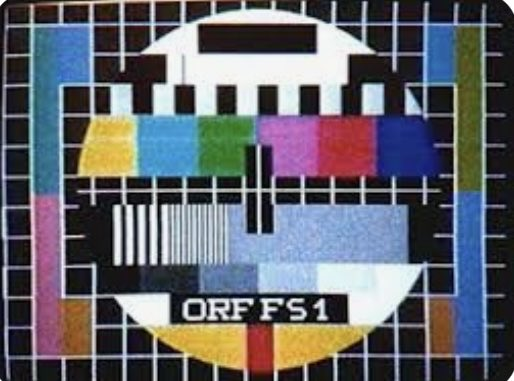
\includegraphics[scale=0.3]{grafik/b1.jpg}
\caption{Analog TV Test}
\end{wrapfigure}
\blindtext



%\blindtext
\end{frame}

  
        %\mode<article>{
    \chapter*{(4) Spule und Induktivität}
    \addcontentsline{toc}{section}{(4) Spule und Induktivität}
}

\begin{frame}{Spule und Induktivität}
\blindtext
\end{frame}

  
        
        %\mode<article>{
        %    \printindex
        %}
    }

\end{document}